
\chapter{Introduction} \label{CH1_Introduction}

\section{Motivation}

The scale of energy demand imposed by modern AI and data center infrastructure extends
far beyond the boundaries of individual facilities.
Figure~\ref{fig:datacenter_energy_footprint} contextualizes this demand across four
dimensions: national-scale electricity consumption, the environmental cost of model
training, per-query inference energy, and the projected growth trajectory driven by AI
adoption.
At the national level, global data centers consumed approximately 415~TWh of electricity
in 2024, a figure comparable to the entire annual electricity consumption of France
(430~TWh) and more than twice that of Sweden (140~TWh), Argentina (130~TWh), or the
Netherlands (120~TWh).
The International Energy Agency projects that this demand will reach approximately
945~TWh by 2030, nearly doubling within six years, as AI-specific server infrastructure
expands at roughly 30\% per year against 9\% for conventional servers.
This trajectory implies that data centers alone will account for approximately 3\% of
total global electricity by the end of the decade, up from 1.5\% today.

\begin{figure}[tbp]
    \centering
    
\includegraphics[width=\textwidth]{Figures/datacenter_energy_footprint.pdf}
    \caption{The energy footprint of AI and data centers at global scale, covering
    national electricity demand comparisons, the environmental cost of model training,
    per-query inference energy ratios, and projected demand growth through 2030.
    Sources: IEA Energy and AI Report 2024; Strubell et al.~(2019).}
    \label{fig:datacenter_energy_footprint}
\end{figure}

The cost of AI is substantial even at the level of a single model.
Training GPT-3 required approximately 1,287~MWh of electricity in a single run,
equivalent to 120 years of an average US household's electricity use, or the annual
CO$_2$ emissions of 112 passenger cars driven for a full year.
The resulting carbon footprint amounts to approximately 552 metric tons of CO$_2$
equivalent for one training run, a figure that grows with each successive generation of
larger and more capable models.
At the inference level, the disparity relative to traditional web services is equally
pronounced: a single ChatGPT (GPT-4) query consumes approximately 0.30~Wh, roughly
7.5 times the energy of a conventional web search query (0.04~Wh).
At the scale of a global user base, aggregate ChatGPT inference amounts to approximately
227~GWh per year, sufficient to power around 20,000 US homes annually.
The combination of high per-query cost and massive query volume means that inference,
not training, now dominates the operational energy footprint of deployed AI systems.
These figures collectively underscore that energy efficiency in data centers and AI
infrastructure is not merely an operational concern for facility managers but a matter
of global resource allocation with direct implications for carbon emissions and energy
security.

Tracing this demand inward, from the global footprint to the individual facility and
ultimately to a single compute node, reveals where efficiency interventions are most
effective.
Data centers are among the most energy-intensive commercial buildings in existence,
consuming between 10 and 50 times more energy per unit floor space than conventional
offices~\cite{darrow2009opportunities,koomey2011growth}.
Globally, they already account for approximately 2\% of total U.S. electricity
consumption, and multiple surveys confirm that power demand growth across datacenter
generations consistently outpaces the efficiency gains delivered by hardware
innovation~\cite{koot2021usage}, making runtime power management an essential complement
to hardware design.
Figure~\ref{fig:datacenter_power_dist} breaks down the facility-level energy budget by
component category, bridging the macro picture of Figure~\ref{fig:datacenter_energy_footprint}
with the node-level view that motivates this dissertation.

\begin{figure}[tbp]
    \centering
    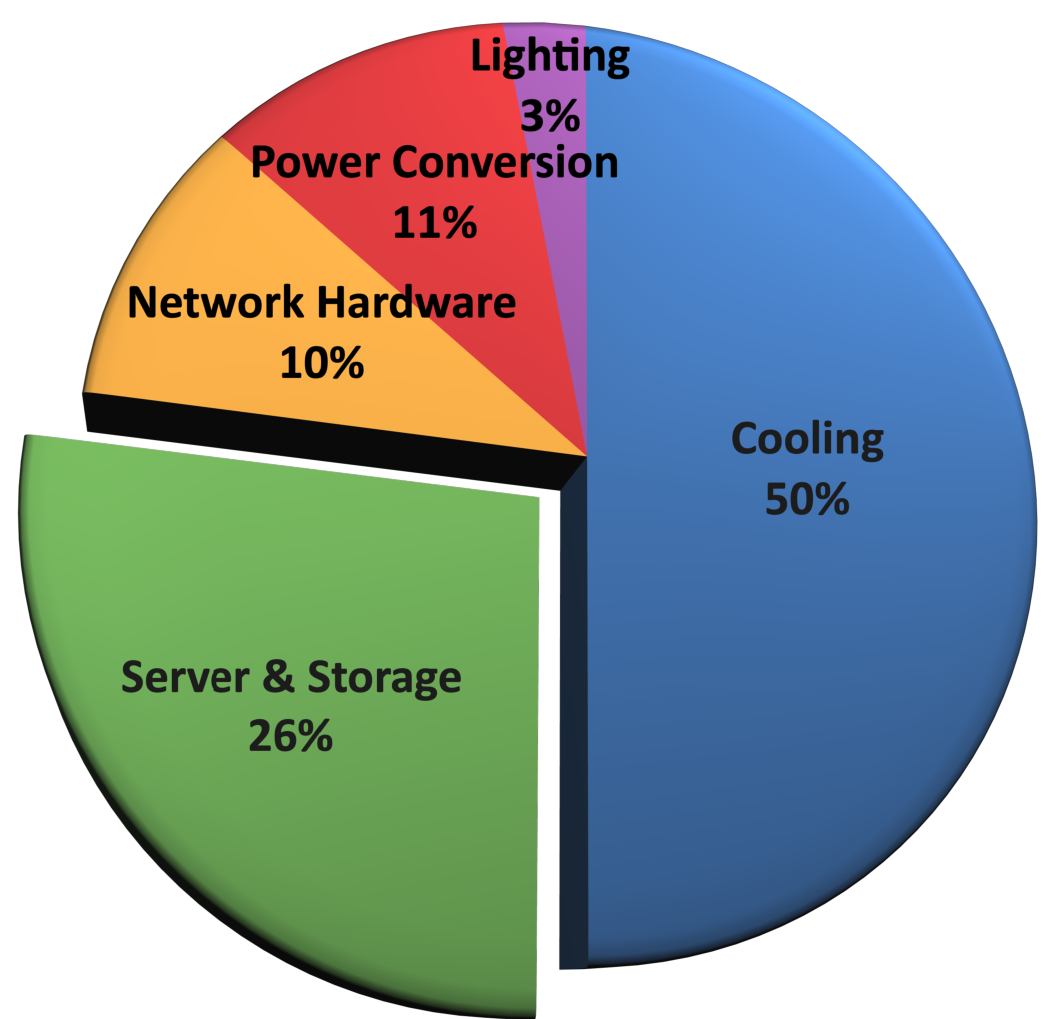
\includegraphics[width=0.55\linewidth]{Figures/datacenter_power_distribution.pdf}
    \caption{Division of consumed power in a typical datacenter. Cooling and
    server and storage hardware together account for 76\% of total power consumption,
    making compute-node power management the highest-leverage target for
    energy efficiency improvements.}
    \label{fig:datacenter_power_dist}
\end{figure}

As shown in Figure~\ref{fig:datacenter_power_dist}, cooling alone accounts for
approximately 50\% of total facility power, while server and storage hardware contributes
a further 26\%, together representing three-quarters of all consumption.
The remaining fraction is distributed across networking infrastructure, power distribution
losses, and lighting.
This distribution identifies compute nodes as the primary lever for efficiency
improvement: they are the second-largest consumer of facility power and the only
subsystem whose energy draw is directly determined by the workload executing on them.
Reducing the power drawn by servers without degrading application performance therefore
has an outsized impact on overall datacenter efficiency.
Crucially, the energy problem does not stop at the facility boundary: within each compute
node, power consumption is itself spatially and temporally uneven, driven by the
fundamental mismatch between processor speed and memory subsystem speed, a source of
inefficiency that neither cooling nor hardware scaling can resolve on its own.

\subsection*{Hardware Architecture and the Origins of Uneven Power Consumption}

Understanding why compute-node power is difficult to control requires examining
the hardware architecture of modern processors.
Figure~\ref{fig:node_hierarchy} shows the memory hierarchy of an Intel Xeon Gold 6240R
processor annotated with the clock-cycle cost at each level.
The most critical architectural mismatch is the speed gap between the processor and the
memory subsystem.
A processor register access requires fewer than one CPU cycle, an L1 cache hit
approximately 4 cycles, an L2 hit approximately 14 cycles, and a main-memory (DRAM)
access approximately 240 cycles.
This two-order-of-magnitude disparity means that the CPU frequently stalls waiting for
data, consuming static power without performing useful computation.

\begin{figure}
    \centering
    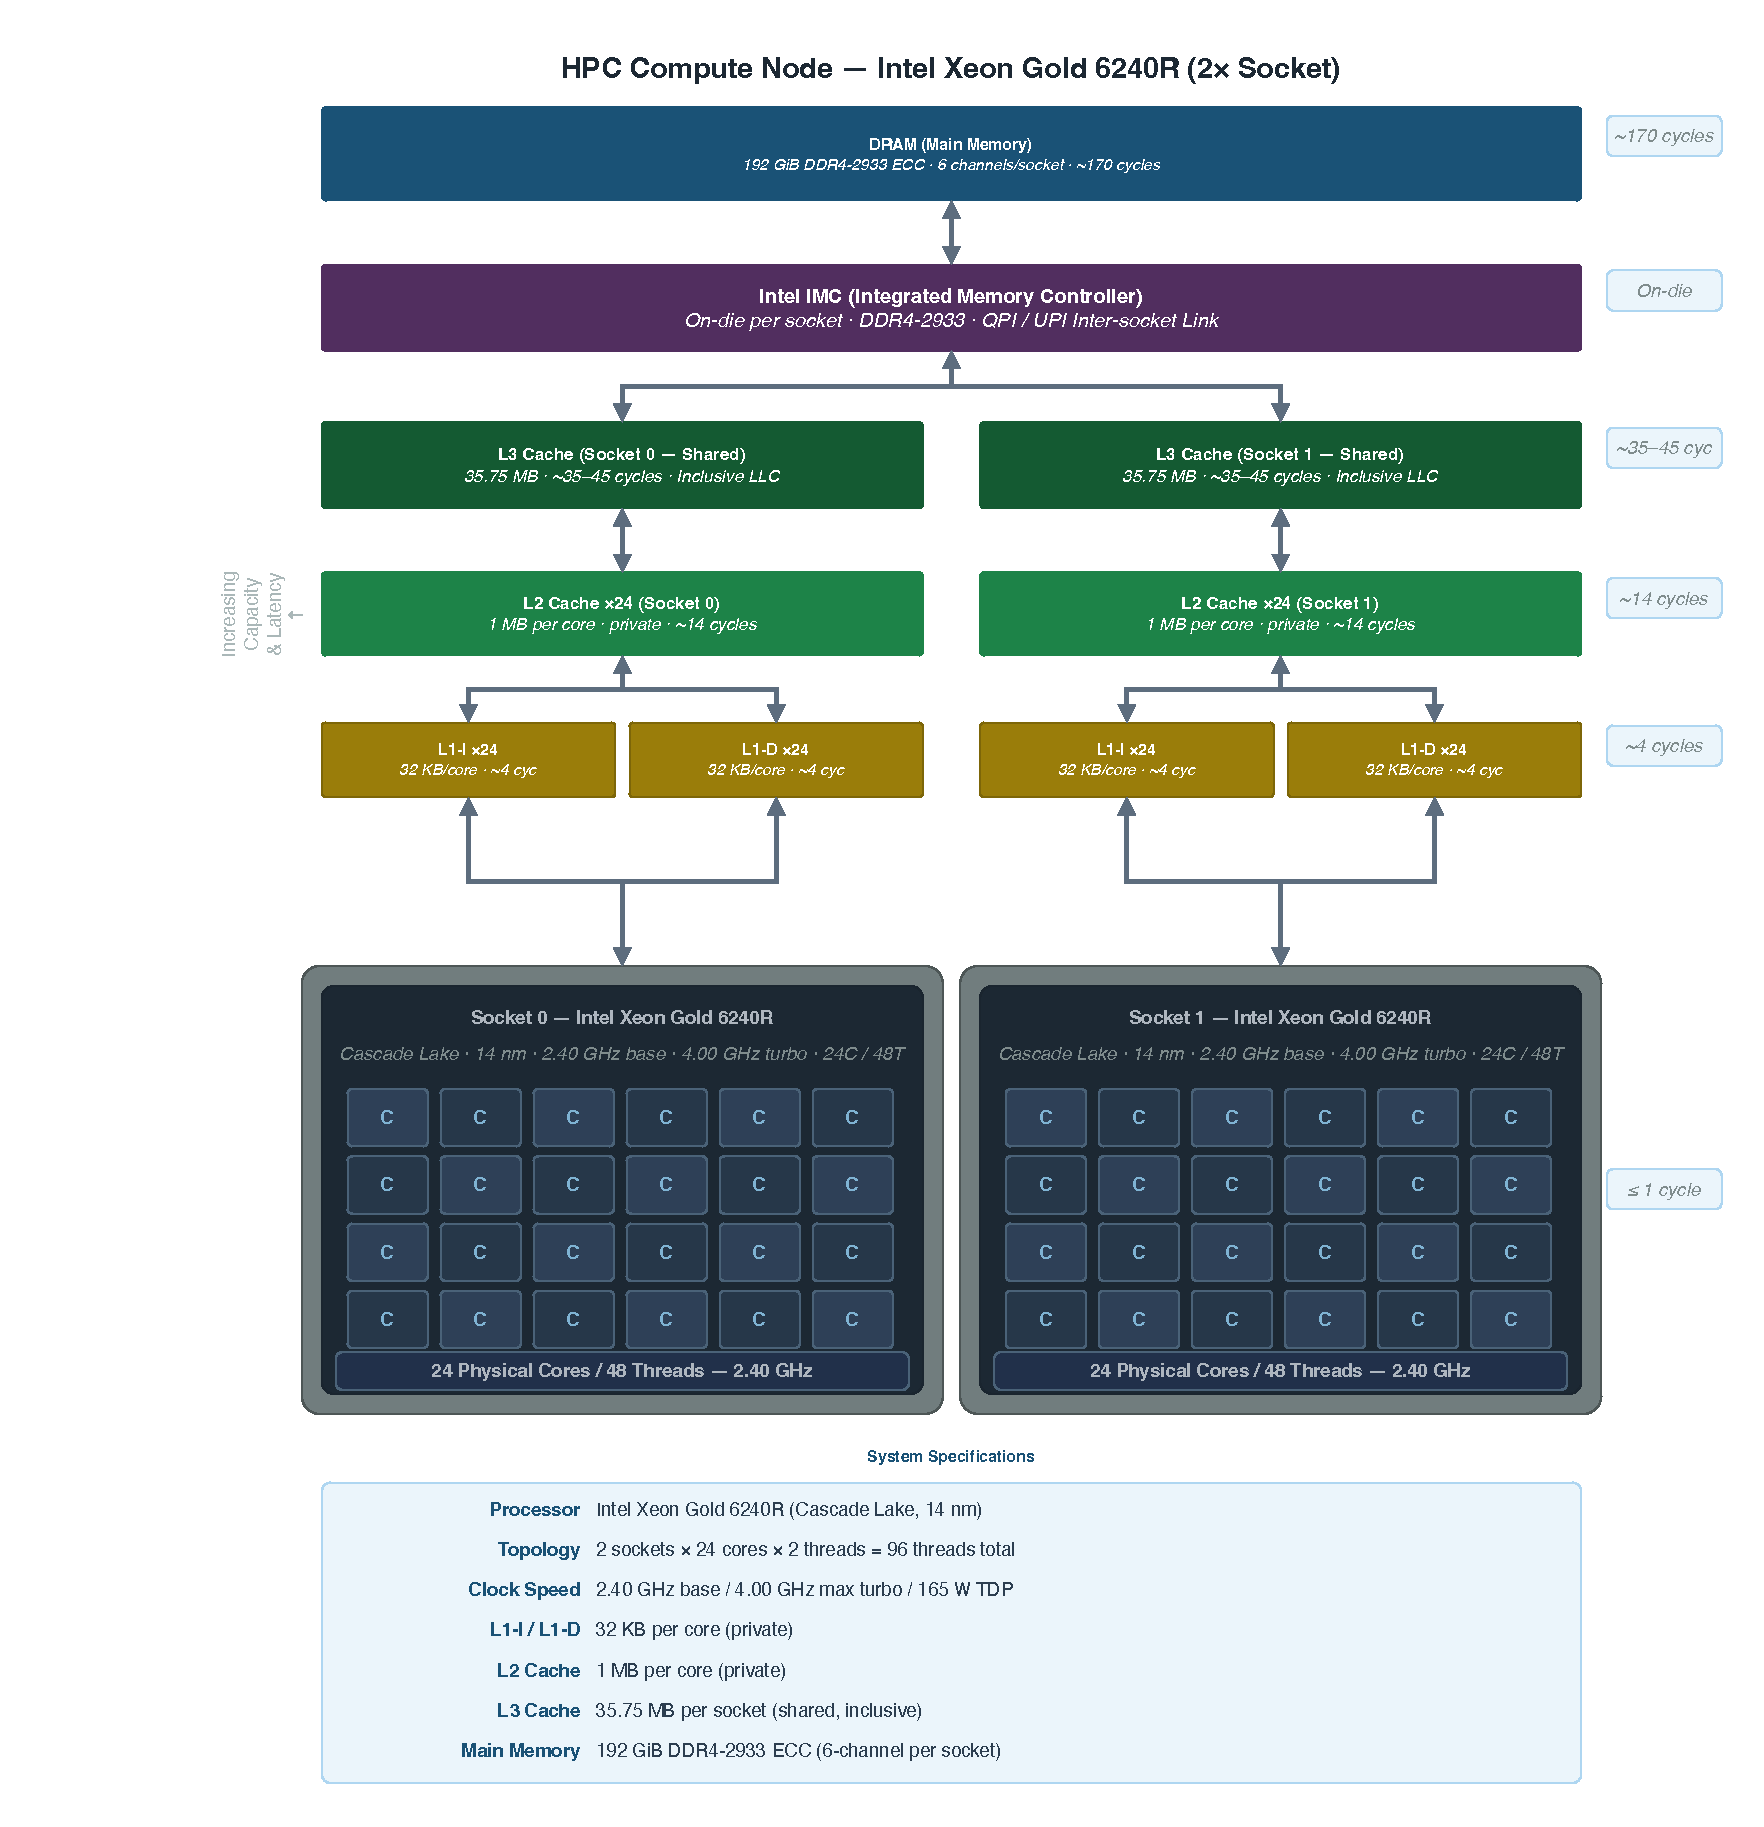
\includegraphics[width=\textwidth, trim={1cm 0cm 0cm 2cm}, clip]{Figures/node_architecture.pdf}
    \caption{Hardware architecture of an Intel Xeon Gold 6240R processor illustrating
    the access latency (in clock cycles) across memory hierarchy levels.
    The figure highlights the increasing cycle cost from the processor core through
    the L1, L2, and L3 caches to DRAM, underscoring the latency bottleneck that arises
    when data must be fetched from main memory during compute-intensive workloads.}
    \label{fig:node_hierarchy}
\end{figure}

The memory hierarchy mixes two fundamentally different storage technologies with opposing
power characteristics.
Static RAM (SRAM), used in on-chip caches, maintains state as long as power is supplied
and offers sub-nanosecond access, but requires constant power to hold state and is
expensive per bit.
Dynamic RAM (DRAM), used in main memory, stores each bit as charge on a capacitor,
making it far cheaper per bit but requiring periodic refresh every 64~ms.
During a refresh cycle, no access to the affected row is possible, stalling the processor.
For some workloads, this refresh overhead can consume up to 50\% of memory-access
cycles~\cite{david2010rapl}.
Every read from DRAM also depletes the capacitor and requires a write-back, adding
further energy overhead.
The cache hierarchy exists precisely to bridge this SRAM--DRAM gap, but the bridging
itself consumes energy in the form of cache fills, evictions, and write-backs.

In multi-socket configurations, the single shared memory bus is replaced by a
Non-Uniform Memory Access (NUMA) topology, where each processor socket has local
memory but can also access the memory of remote sockets via an interconnect.
The energy and latency cost of a memory access then depends on whether the data resides
in local or remote memory: local accesses are cheaper, while remote accesses traverse
the inter-socket interconnect at significantly higher latency and energy cost.
This means that identical workloads running on different cores can consume different
amounts of energy depending solely on data placement, a fundamental asymmetry that
neither software nor hardware resolves automatically.
Multi-core cache sharing further adds coherence overhead: when one core writes to a
cache line, all other cores holding a copy must invalidate their copy, and dirty cache
lines being evicted must be written back to main memory, activating the full memory
path at high energy cost.
The combined result is that power consumption is uneven both spatially (across
components) and temporally (across workload phases), which makes static power
budgets highly inefficient.

\subsection*{The Need for Adaptive Power Management}

Modern processors expose hardware actuators specifically designed to address this
challenge.
Interfaces such as Intel's Running Average Power Limit (RAPL)~\cite{david2010rapl} and
Dynamic Voltage and Frequency Scaling (DVFS)~\cite{4658633} allow software to set
per-domain power caps and adjust processor frequency at runtime.
However, simply capping power at a fixed level is insufficient: the relationship between
power and application performance is non-linear.
There exist operating regions in which similar performance levels are achieved at
substantially lower power, and identifying these regions requires observing the
application's runtime behavior~\cite{czarnul2019energy}.

Existing power management approaches can be broadly classified as hardware-centric
or application-specific.
Hardware-centric schemes optimize power dissipation at the circuit level and are not
aware of application semantics, while application-specific methods require
re-parameterization whenever the application or hardware platform changes.
Neither class of approach is sufficient for the heterogeneous, multi-tenant HPC
environments of today, where hundreds of distinct applications share the same physical
infrastructure.
What is needed is a controller that is simultaneously hardware-agnostic (requiring no
prior knowledge of the processor architecture) and application-agnostic (requiring no
deep characterization of the specific workload), yet still capable of adapting its
decisions to the instantaneous performance of the running application.

\subsection*{Reinforcement Learning for Energy-Efficient HPC}

Reinforcement learning (RL) offers a principled framework for designing such adaptive
controllers.
An RL agent observes the state of the system at each time step, takes an action (in
this context, adjusting the power cap), and receives a reward signal that encodes the
trade-off between energy consumption and application performance.
Over time, the agent learns a policy that maximizes cumulative reward, i.e., one that
achieves high energy savings without unacceptable performance loss.

The first step in this direction, presented in Chapter~\ref{CH3_IC2E}, is an
online RL framework that trains a Proximal Policy Optimization (PPO) agent using a
mathematical model of the compute node, capturing the relationship between the applied
power cap and the application's instantaneous progress toward its scientific objective.
By training on this lightweight surrogate model rather than on the live system, the
approach avoids the risk of degrading production workloads during exploration.
The controller is deployed through the RAPL interface and demonstrated on an Intel
Cascade Lake node using the STREAM benchmark.

While model-based online RL establishes the feasibility of RL-driven power management,
it still requires constructing a surrogate model for each new hardware platform.
Chapter~\ref{CH4_HPDC} advances the approach by eliminating this requirement entirely
through offline RL: the agent is trained on pre-collected execution traces gathered
under arbitrary policies, with no live interaction with the target system during
training.
This offline formulation enables policy development for new platforms without access to
those platforms, and the resulting controller is validated across twelve benchmark
applications spanning memory-bandwidth-bound and compute-bound workloads, achieving
an average energy reduction of 20\% with only 7.4\% average performance loss.

A remaining challenge in both of the above approaches is that they produce a single
fixed policy for a given energy-performance trade-off.
In practice, different users and different jobs have different tolerance for performance
degradation, and deploying a separate RL agent for each desired operating point is
impractical.
Chapter~\ref{CH5_ICS} addresses this through the Decay-Driven Multi-Objective
Reinforcement Learning (DDMORL) framework, a single offline-trained controller that
accepts a user-specified maximum performance degradation as input and produces
the corresponding power-cap schedule.
This eliminates the need for multiple agents or manual weight tuning and generates
well-structured Pareto fronts in the energy-degradation trade-off space.

\subsection*{Edge-to-HPC: Extending the Continuum}

Energy efficiency in HPC cannot be considered in isolation from the broader scientific
computing ecosystem.
Large-scale scientific experiments increasingly rely on an integrated edge-to-HPC
continuum, where data is generated at remote sensors or instruments, processed at the
edge to reduce volume, and then forwarded to HPC systems for full-scale simulation
and analysis.
Edge computing at the source lowers the need to transmit raw data to the HPC center,
reduces latency, and enables immediate feedback to scientists as experiments unfold.
Equally, AI models deployed at the edge can be retrained with new experimental data
using the computing resources of connected HPC systems, allowing workflows to adapt as
new scientific needs arise.

This edge-to-HPC integration, however, brings its own resource management challenges.
Application runs and data processing at the edge are typically executed and curated
manually, with resource requirements that are neither automatically adjusted nor
propagated across the continuum.
Chapter~\ref{CH6_Charon} addresses this gap with the Charon framework, which
investigates how edge resources can be arbitrated dynamically under a user-provided
performance goal, how system software can support AI-at-the-edge applications that
leverage HPC platforms for model tuning, and how flexible user-agnostic system software
policies can be deployed across diverse hardware setups and use cases.

Together, the contributions in this dissertation span the full stack of energy-aware
scientific computing: from low-level, per-node power control under hardware constraints,
to high-level, edge-to-HPC workflow management under real-time scientific demands.

\section{Research Contributions}

\begin{enumerate}

    \item \textbf{Online RL for Performance-Aware Power Management (Chapter~\ref{CH3_IC2E}):}
    A reinforcement learning approach for dynamic power capping of HPC compute nodes
    using the Intel RAPL interface, trained with a Proximal Policy Optimization (PPO)
    agent on a mathematical model of compute node behavior and validated using the
    STREAM benchmark.

    \item \textbf{Offline RL for Application-Agnostic Energy Efficiency (Chapter~\ref{CH4_HPDC}):}
    An offline RL-based power controller trained on pre-collected execution traces,
    capable of learning an application-agnostic energy efficiency policy without
    requiring online interaction with the target system. The approach is validated
    across multiple benchmarks spanning memory-bandwidth-bound and compute-bound
    workloads.

    \item \textbf{Decay-Driven Multi-Objective RL for Energy Efficiency (Chapter~\ref{CH5_ICS}):}
    The Decay-Driven Multi-Objective Reinforcement Learning (DDMORL) framework, a
    single offline-trained controller that allows users to specify their maximum
    tolerable performance degradation as a percentage. The framework eliminates the
    need for multiple agents or manual preference tuning and produces well-structured
    Pareto fronts in the energy-degradation trade-off space.

    \item \textbf{Edge-to-HPC Resource Management (Chapter~\ref{CH6_Charon}):}
    The Charon framework for dynamic arbitration of edge computing resources under
    user-provided performance goals, enabling adaptive scientific workflows that
    span edge devices and HPC platforms within an integrated computing continuum.

\end{enumerate}

\section{Dissertation Organization}

The remainder of this dissertation is organized as follows.
Chapter~\ref{CH2_LiteratureReview} surveys the relevant background: the physical limits
driving HPC power constraints, the hardware actuators and software runtimes used to
manage power, and the performance proxies that close the feedback loop.
Chapter~\ref{CH3_IC2E} presents the first reinforcement learning approach for
dynamic, online power capping of HPC compute nodes using Intel RAPL.
Chapter~\ref{CH4_HPDC} advances this with an offline RL-based, application-agnostic
energy efficiency controller validated across a diverse set of benchmarks.
Chapter~\ref{CH5_ICS} introduces the DDMORL framework for preference-driven,
multi-objective energy-performance trade-off control.
Chapter~\ref{CH6_Charon} broadens the scope to edge-to-HPC workflows, presenting
the Charon framework for dynamic edge resource management in scientific computing
continua.
Each chapter is self-contained, presenting the motivation, methodology, experimental
evaluation, and conclusions of the corresponding research contribution.
